%-----------------------------------------------------------------------------------------
%  Dieses Projekt wurde erstellt mit der LaTeX Vorlage von Jonas Bingel
%  Die LaTeX Vorlage kann heruntergeladen werden unter: github.com/JonasBingel/HSMZ-Thesis-Template
% -----------------------------------------------------------------------------------------

% Erklärender Text zu dieser Datei --------------------------------------------------------
% Die Datei Thesis.tex ist die Hauptdatei, die dem LaTeX-Kompiler übergeben wird.
% Diese Datei ist zu verwenden, wenn die eigentliche Haus/Bachelor/Masterarbeit erstellt werden soll.
% In dieser Datei wird 
%  - das Dokument erstellt und alle anderen tex-Dateien werden geladen.
%  - die .bib-Datei eingebunden zur Bereitstellung der Quellen
%  - die Struktur des Dokuments wird definiert
% -----------------------------------------------------------------------------------------

\documentclass[
english, % ngerman für neue Deutsche Rechtschreibung
headings=normal, % normale Headings
captions=tableheading, % Positioniert Captions über Tabellen
listof=totoc,
bibliography=totoc,
%usegeometry, % Auskommentieren wenn Package geometery verwendet wird
overfullrule, % entfernen nach abschluss der bearbeitung
% Default Values, die scrreprt nutzt
%oneside, % Einseitige Seitengenerierung
%11pt, % Font size
% a4paper, % paper
]{scrreprt}
\KOMAoptions{%
  DIV=12,
  parskip=half*,
% %BCOR=korrektur, % absoluter Wert der Bindekorrektur
}

\input{00_General/Metadata}
\input{00_General/Packages}
\input{00_General/Commands}

% Typesetting options
\widowpenalty=10000     % Hurenkinder
\clubpenalty=10000      % Schusterjungen



\addbibresource{sample.bib}
% Wegen dem folgenden Befehl werden im Literaturverzeichnis alle Quellen gelistet, die in der .bib Datei enthalten sind. 
% Wird der Befehl entfernt, werden nur die Quellen gelistet, die auch zitiert werden.
% Der Befehl sollte bei Abgabe der Bachelorarbeit entfernt werden.
\nocite{*} 
\newcounter{romanConsecutive}

\begin{document}
\include{00_General/ToDo}

\pagestyle{empty}
\renewcommand*{\chapterpagestyle}{empty}
% Erklärender Text zu dieser Datei --------------------------------------------------------
% Die Datei 01_EmbargoNotice.tex dient der Definition eines optionalen Sperrvermerks, der vor der Arbeit
% Der derzeit dargestellte Sperrvermerk entspricht der Vorgabe der HS Mainz und wird mit Angaben aus Metadata.tex gefüllt
% -----------------------------------------------------------------------------------------
\pdfbookmark{Sperrvermerk}{sperrvermerk}
\addchap*{Sperrvermerk}
Die vorliegende \art mit dem Titel \titel enthält interne und vertrauliche Daten des Unternehmens/der Einrichtung \unternehmen.

Die \art darf nur den Gutachtern (insbesondere Erst- und Zweitgutachtern), den Mitgliedern der Prüfungsorgane (einschließlich Beisitzer \& Plagiatskontrolle) sowie den in einem eventuellen Rechtschutzverfahren Betrauten zugänglich gemacht werden.

Im Übrigen ist eine Veröffentlichung und Vervielfältigung der Abschlussarbeit -- auch in Auszügen -- nicht gestattet. Vorbehaltlich der Vorschriften zum Prüfungsverfahren und der Prüfung bedarf eine Einsichtnahme in die Arbeit durch Dritte einer ausdrücklichen Genehmigung der Verfasserin/des Verfassers sowie des \oa Unternehmens.

Diese Geheimhaltungsverpflichtung gilt bis zum Ablauf des \datumAblaufSperrvermerk.

\include{01_FrontMatter/02_TitlePage}
% Erklärender Text zu dieser Datei --------------------------------------------------------
% Die Datei 03_Declaration.tex dient der Definition der Eidesstattlichen Erklärung.
% Die Datei enthält den Text, der im Leitfaden der Hochschule Mainz vorgegeben ist.
% Außerdem enthält die Datei die Angaben zur, mit der Betreuenden Person vereinbarten, KI-Nutzung. Hier muss die korrekte Angabe auskommentiert werden
% Wenn ein Bild einer Unterschrift eingefügt werden soll, ist an der Stelle %TODO dem Hinweis zu folgen.
% -----------------------------------------------------------------------------------------
\pdfbookmark{Eigenständigkeitserklärung}{eigenstaendigkeitserklaerung}
\addchap*{Eigenständigkeitserklärung}

Hiermit versichere ich,

\vspace{0.5em}

Name, Vorname: \autorNachname, \autorVorname,

\vspace{0.5em}

dass ich die anliegende Arbeit

\vspace{0.5em}

Titel der Arbeit: \titel \\
Studienfach: \studiengang \\
Prüfer/in: \betreuer

\vspace{0.5em}

selbst angefertigt und alle für die Arbeit verwendeten Quellen und Hilfsmittel in der Arbeit vollständig angegeben habe. Zudem versichere ich, dass ich weder diese noch inhaltlich verwandte Arbeiten als Prüfungsleistung in anderen Fächern eingereicht habe oder einreichen werde.

\vspace{0.5em}


Ich versichere außerdem, 

% TODO eine der folgenden Optionen ist mit der Prüfenden Person abzustimmen und entsprechend auszukommentieren.

\vspace{0.5em}

%Option 1: Erlaubnis von KI-Tools mit geringfügiger Dokumentation
dass ich die Nutzung aller für die Erstellung dieser Arbeit erlaubten generativen KI-Tools im Anhang der vorliegenden Arbeit durch die Benennung des Tools und seines Einsatzzwecks tabellarisch dokumentiert habe. Alle wortwörtlich übernommenen oder paraphrasierten Inhalte von generativen KI-Tools wurden entsprechend gekennzeichnet. Mir ist bewusst, dass der Versuch einer nicht-dokumentierten Nutzung generativer KI-Tools als Täuschungsversuch entsprechend der Prüfungsordnung zu werten ist. Ich versichere, dass ich die mithilfe von KI-Tools generierten Inhalte nicht unreflektiert übernommen habe und ich als Autor:in die Verantwortung für Angaben und Aussagen in dieser Arbeit trage.

%Option 2: Erlaubnis von KI-Tools mit umfangreicher Dokumentation
%dass ich die Nutzung aller für die Erstellung dieser Arbeit erlaubten generativen KI-Tools im Anhang der vorliegenden Arbeit tabellarisch dokumentiert habe. Dazu gehört, welche generativen KI-Tools für welchen Zweck verwendet habe und auf welche Ausschnitte der Arbeit sich diese Nutzung bezieht. Ich habe zudem alle, von dem / der Prüfer:in angeforderten Quellen (Prompts \& Outputs), die meinen Einsatz von generativen KI-Tools bei der Erstellung dieser Arbeit nachweisen, nach bestem Wissen im Anhang der Arbeit zur Verfügung gestellt. Alle wortwörtlich übernommenen oder paraphrasierten Inhalte von generativen KI-Tools wurden entsprechend gekennzeichnet. Mir ist bewusst, dass der Versuch einer nicht-dokumentierten Nutzung generativer KI-Tools als Täuschungsversuch entsprechend der Prüfungsordnung zu werten ist. Ich versichere, dass ich die mithilfe von KI-Tools generierten Inhalte nicht unreflektiert übernommen habe und ich als Autor:in die Verantwortung für Angaben und Aussagen in dieser Arbeit trage.

%Option 3: Verbot von KI-Tools
%dass ich keine auf Künstlicher Intelligenz (KI) basierenden Text- oder Bildgeneratoren (z.\,B.\ ChatGPT) verwendet habe, da der Einsatz dieser Tools bei der Erstellung dieser Arbeit mir durch den / die Prüfer:in explizit verboten wurde. Mir ist bewusst, dass der Einsatz eines generativen KI-Tools eine Missachtung der Vorgabe ist und dies als Täuschungsversuch entsprechend der Prüfungsordnung gewertet wird.

\vspace{3em}

\noindent
\begin{tabular*}{\linewidth}{p{0.5\linewidth}p{0.5\linewidth}}
  	\ort, den \datumAbgabe &
  	%TODO Wenn eine Unterschrift eingefügt werden soll, muss nachfolgender Kommentar eingefügt und die Zeile darunter auskommentiert werden.
      % Einfuegen der Unterschrift als Datei "signature.png". Height muss ggf. angepasst werden.
  	% \makebox[\linewidth][l]{
      %   \includegraphics[height=1.2cm]{04_Artifacts/01_Figures/signature.png}
  	% }
  	\autor
  	\\[1em]
  	Ort, Datum & Unterschrift
\end{tabular*}

% Erklärender Text zu dieser Datei --------------------------------------------------------
% Die Datei 04_ManagementSummary.tex dient der Definition der Management Summary.
% Wenn statt dem Bezeichner Management Summary der Begriff "Abstract" verwendet werden soll, ist in den mit %TODO gekennzeichneten Zeilen "Management Summary" durch "Abstract" zu ersetzen.
% -----------------------------------------------------------------------------------------
\pdfbookmark{Abstract}{abstract} %TODO ggf. durch Management Summary ersetzen
\addchap*{Abstract} %TODO ggf. durch Management Summary ersetzen
% Blindtext, damit die Abstract Seite gefüllt wird - diesen natürlich später entfernen
\blindtext[3]

\pagestyle{plain}
\renewcommand*{\chapterpagestyle}{plain}
\pagenumbering{Roman}
% Erklärender Text zu dieser Datei --------------------------------------------------------
% Die Datei 05_Lists.tex dient der Definition der zu generierenden Verzeichnisse und deren Reihenfolge.
% Wenn einzelne Verzeichnisse nicht generiert werden sollen, sind die entsprechenden Anweisungen auszukommentieren.
% -----------------------------------------------------------------------------------------

% Inhaltsverzeichnis ----------------------------------------------------------------------
\pdfbookmark{Table of Contents}{tableofcontents}
\tableofcontents

% Abbildungsverzeichnis -------------------------------------------------------------------
\listoffigures

% Tabellenverzeichnis ---------------------------------------------------------------------
\listoftables

% Abkuerzungsverzeichnis ------------------------------------------------------------------

\newcommand{\abbr}{List of Abbreviations}
\chapter*{\abbr}
\addchaptertocentry{}{\abbr}
\input{01_FrontMatter/06_Abbreviations}

% Symbolverzeichnis -----------------------------------------------------------------------
\printnomenclature

% Formelverzeichnis -----------------------------------------------------------------------
\listofequations

% Listingverzeichnis ----------------------------------------------------------------------
\listoflistings

% Algorithmenverzeichnis ------------------------------------------------------------------
\listofalgorithms

\include{00_General/Nomenclature}

\setcounter{romanConsecutive}{\value{page}}
\pagenumbering{arabic}
\include{02_MainText/00_ThesisContent}

\pagenumbering{Roman}

\setcounter{page}{\value{romanConsecutive}}
\printbibliography[title={Literaturverzeichnis}]
% Erklärender Text zu dieser Datei --------------------------------------------------------
% Die Datei 01_Appendix.tex dient der Definition des Anhangs und dessen Reihenfolge.
% -----------------------------------------------------------------------------------------
\appendix
\clearpage
\pdfbookmark{Anhang}{anhang}
\chapter{Anhang Listing}
\addcontentsline{toc}{chapter}{Anhang}

% Anhang nachfolgend einfügen ----------------------------------------------------------------------

\begin{longlisting}
\label{app:longlisting}
\caption{Langes Listing in Java}
\label{listing:longlisting}
\inputminted{java}{04_Artifacts/03_Listings/Data.java}
\end{longlisting}

\chapter{Anhang Auszug PDF}
\label{app:auszugPDF}
\begin{figure}[h]
    \centering
    \frame{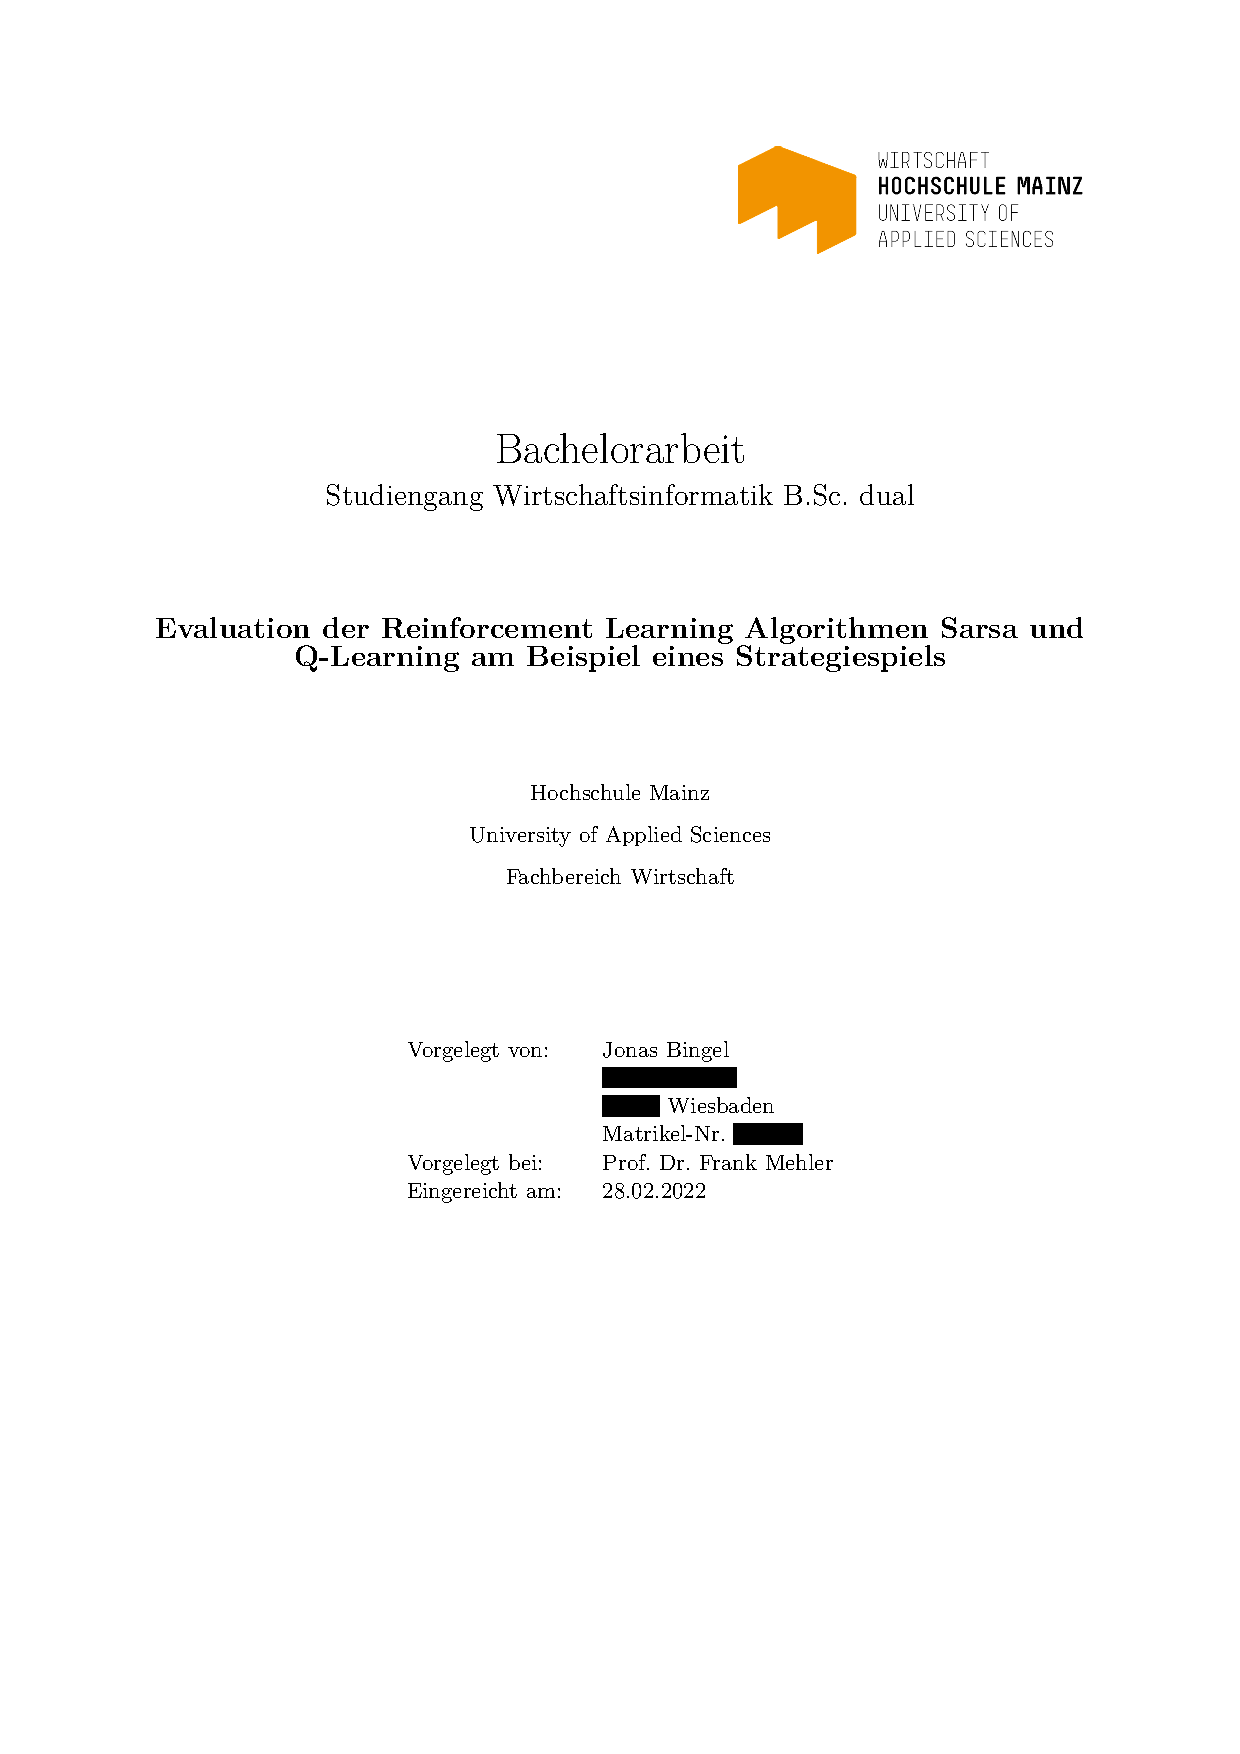
\includegraphics[width=0.7\linewidth]{04_Artifacts/SamplePDF.pdf}}
    \caption[Beispiel für den Auszug aus einer PDF]{Beispiel für den Auszug aus einer PDF im Anhang}
\end{figure}

\chapter{Anhang Tabelle}
\label{app:longtable}
\input{04_Artifacts/02_Tables/LongSample}


\usestandardtocs
\bookmarksetup{startatroot}% siehe bookmark-Anleitung

\end{document}
